\vspace{-0.7em}
\section{Refusal Index}
\vspace{-0.7em}
\label{sec:refusal_index_method}

% We begin by defining the scope and objective of our research. When evaluating calibration, we want to measure whether, higher confidence in model answers leads to a higher accuracy. More precisely, whether the model's output probability aligns with the actual probability of being correct. However, evaluating either probability or correctness for arbitrary text outputs remains an open problem, as ground truth can be subjective, non-deterministic, or unavailable.

% \noindent\textbf{Problem.}
% Measuring an LLM's ability to refuse questions beyond its knowledge presents several challenges.
% On the one hand, refusal decisions are not solely determined by a model's self-knowledge. 
% Instead, model preferences, question risk levels, or explicit instructions can influence these decisions. 
% Consequently, these factors preclude simply counting refusal rates to evaluate knowledge-aware refusal. 
% For example, a model designed with a higher refusal tendency will easily achieve a higher score when measured with refusal rate on unanswerable questions, regardless of its actual knowledge.
% On the other hand, we cannot rely on external calibrators like verbalized confidence~\citep{xiong2023can} or linear probe to replace direct refusal measurements, because these calibrators may not accurately reflect a model's internal self-knowledge about when to refuse.
% Therefore, an effective metric for knowledge-aware refusal must: (1) quantify knowledge-aware refusal accurately, (2) remain consistent across different refusal rates, and (3) derive directly from black-box LLM outputs.

\noindent\textbf{Scope.} 
Our evaluation settings follow widely used factuality evaluations like SimpleQA and TruthfulQA~\citep{wei2024measuringshortformfactualitylarge, lin2022truthfulqameasuringmodelsmimic}, where models provide atomic answers for short-form, factual questions. 
Additionally, models can refuse to answer to avoid hallucination by producing outputs such as \emph{``I don't have enough information...''}.
Following SimpleQA, each model answer is classified as correct, incorrect, or refused by comparing it against the ground truth. 
The classification results are used to estimate the model's factuality level, or in our case, the ability to make knowledge-aware refusals.
This formulation avoids subjective grading and partial correctness in LLM generation, allowing more reliable measurement.

\noindent\textbf{Notations.}
Formally, we denote the LLM as $f_{\text{LM}}: \mathcal{X} \rightarrow \mathcal{Y} \cup \{\bot\}$, where $x \in \mathcal{X}$ represents the input question, $y \in \mathcal{Y}$ represents the output answer, and $\bot$ denotes refusal. 
For the $i$-th question $x_i$ with ground truth $y_i$ in dataset $D$, we define two indicators: $W_i = \mathbf{1}\{f_{\text{LM}}(x_i) \neq y_i\}$ for incorrect outputs (including refusals) and $R_i = \mathbf{1}\{f_{\text{LM}}(x_i) = \bot\}$ for refusal responses. 
We define the error probability $w_i = P(f_{\text{LM}}(x_i) \neq y_i)$ and the refusal probability $r_i = P(f_{\text{LM}}(x_i) = \bot)$. 
Conceptually, a model with better knowledge-aware refusal should refuse more frequently as questions become more difficult. 
We measure this ability with the \emph{Refusal Index}. 
Inspired by rank-based calibration metrics like AUROC~\citep{NiculescuMizil2005PredictingGP}, we define the Refusal Index as the correlation between refusal probabilities and error probabilities:

\begin{definition}[Refusal Index]
Refusal Index $\rho_S$ is defined as Spearman's rank correlation between the model's refusal probability $r_i$ and the error probability $w_i$ as follows:

\vspace{-1em}
\begin{equation}
   \text{Refusal Index} = \rho_S  = \text{Corr}(\text{Rank}(r_i), \text{Rank}(w_i)).
\end{equation}
\vspace{-1.5em}

\end{definition}

The intuition behind the definition is that a model achieves \emph{perfect knowledge-awareness} when its refusal probability increases monotonically with error probability, making it more likely to refuse as questions become more difficult:

\vspace{-1em}
\begin{equation}
w_i \leq w_j \iff P(f_{\text{LM}}(x_i) = \bot) \leq P(f_{\text{LM}}(x_j) = \bot).
\label{eq:refusal_perfect_calibrated}
\end{equation}
\vspace{-1.5em}

Note that this differs from error-based calibration metrics like Expected Calibration Error (ECE), which quantify absolute discrepancies between $r_i$ and $w_i$. 
In contrast, our approach evaluates only the rank discrepancies between $r_i$ and $w_i$.
We define RI as a discrimination property because it captures the fundamental aspect of knowledge-aware refusal. 
This is because absolute discrepancy-based metrics are sensitive to changes in a model's overall refusal rate, which can significantly affect the metric value (an undesirable property). 
In contrast, discriminative metrics like RI or AUROC measure only the rank between different samples, making them more robust to changes in overall refusal rates. 
Alternatively, it is generally easier for a model to adjust its overall refusal rate than to improve its ability to rank questions by difficulty accurately.
Next, we introduce how to estimate the Refusal Index through a two-pass evaluation process (\Secref{sec:two_pass_evaluation}).


\vspace{-0.5em}
\subsection{Two-Pass Evaluation}
\vspace{-0.5em}
\label{sec:two_pass_evaluation}

The naive way to measure RI would require the refusal probability $P(f_{\text{LM}}(x_i) = \bot)$ across questions with varying error probabilities. 
However, in factuality evaluation, we only observe single text output from the model, making refusal probabilities inaccessible. 
To address this issue, we propose a two-pass evaluation process to infer the Spearman correlation between refusal and error probabilities from binary observations. 
This approach models refusal decisions by first treating refusal and correctness indicators as results of thresholding on their respective probabilities, and then modeling their joint distribution with a Gaussian copula. 


\noindent\textbf{Formulating the Joint Distribution.} We estimate $\rho_S$ from the joint distribution of refusal and error probabilities using a Gaussian copula model with correlation $\rho$ as follows:

\vspace{-1em}
\begin{equation}
C(u,v) = \Phi_\rho\!\big(\Phi^{-1}(u), \Phi^{-1}(v)\big).
\end{equation}
\vspace{-1.5em}

Here, $u = F_r(r_i)$ and $v = F_e(w_i)$ are the marginal CDFs, $\Phi^{-1}$ is the standard normal quantile function, and $\Phi_\rho$ is the bivariate standard normal CDF with correlation $\rho$. 
This Gaussian copula specifies only the dependence on $\rho$ and leaves the marginal distributions of $r_i$ and $w_i$ unrestricted. 
The function $\Phi_\rho$ depends only on rank correlation, remaining independent of the marginal distributions. 
Next, we avoid modeling $F_r$ and $F_e$ directly and instead estimate $\rho$ from $R_i$ and $W_i$ via maximum likelihood. 
We then compute $\rho_S$ from $\rho$ using the standard conversion formula for Gaussian copulas: $\rho_S = \frac{6}{\pi}\arcsin\!\left(\frac{\rho}{2}\right)$~\citep{kendall1979advanced}. 
Because $\rho$ determines the corresponding rank correlations of $r_i$ and $w_i$ via a monotonic transformation, we could equivalently report other rank measures such as Kendall's $\tau$ instead of $\rho_S$. We use Spearman's $\rho$ for interpretability.

\begin{wrapfigure}{r}{0.5\textwidth}
    \vspace{-1em}
    \centering
    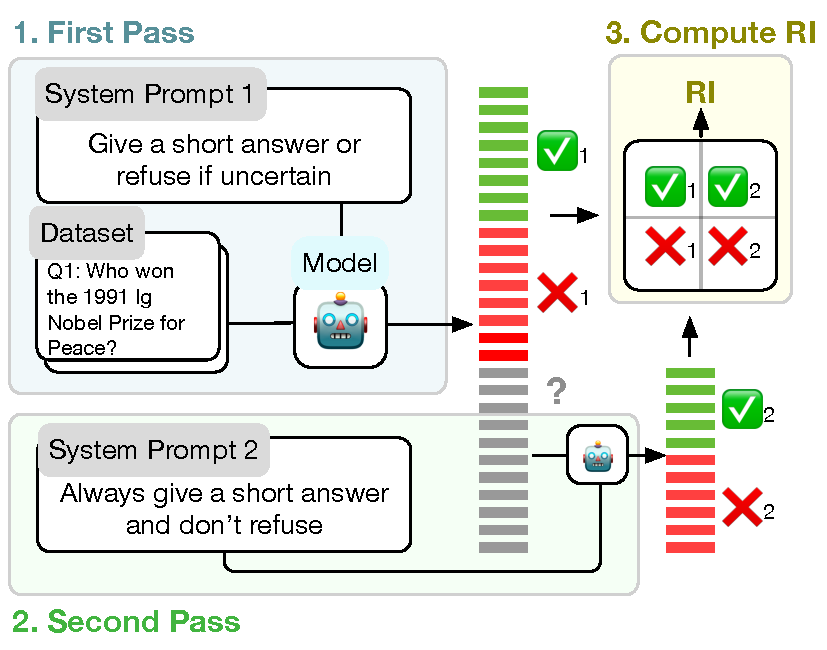
\includegraphics[width=0.45\textwidth]{Figures/two-pass.pdf}
    \caption{Illustration of two-pass evaluation process.}
    \label{fig:two_pass_evaluation}
    \vspace{-1.5em}
\end{wrapfigure}

Estimating $\rho$ requires observing two binary indicators for each sample: $R_i$ for refusal probability $r_i$ and $W_i$ for error probability $w_i$, while $r_i$ and $w_i$ themselves remain latent. 
We achieve this through a two-pass evaluation that runs the model on the same dataset twice. 
The first pass observes refusal decisions $R_i$, using a standard setup that allows the model to answer or refuse each question, classifying responses as correct, incorrect, or refused. 
The second pass observes correctness $W_i$ by updating the system prompt to remove abstention options and requiring the model to answer all questions. We provide prompt details in \Secref{app:system_prompts} and an illustration in \Figref{fig:two_pass_evaluation}.
We run the second pass only on questions refused in the first pass, collecting correctness indicators $W'_i$ for all refused questions ($R_i = 1$).

\noindent\textbf{Estimating Refusal Index.} We define the aggregated correctness indicator $\hat{W}_i = R_i \cdot W'_i + (1-R_i) \cdot W_i$ as the correctness when the model provided an answer. 
The empirical refusal rate is $r=\sum_{i=1}^{|D|} R_i/|D|$ and the error rate is $\mu = \sum_{i=1}^{|D|} \hat{W}_i/|D|$. 
Under our model, the pair $(R,\hat{W})$ results from thresholding a bivariate standard normal vector $(Z_R,Z_W)$ with correlation $\rho$ at, matching the standard tetrachoric setup implied by the copula.


\vspace{-1em}
\begin{equation}
    \begin{aligned}
        \tau_R=\Phi^{-1}(1-r), \qquad \tau_W=\Phi^{-1}(1-\mu).
    \end{aligned}
\end{equation}
\vspace{-1.5em}

Let $n_{ab}$ be the counts of $(R=a, \hat{W}=b)$ for $a,b\in\{0,1\}$. The cell probabilities are

\vspace{-1em}
\begin{equation}
    \begin{aligned}
    p_{11}(\rho) &= \bar\Phi_2\!\big(\tau_R,\tau_W;\rho\big) \;=\; P(Z_R>\tau_R, Z_W>\tau_W),\\
    p_{10}(\rho) &= r - p_{11}(\rho),\qquad
    p_{01}(\rho) \;=\; \mu - p_{11}(\rho),\\
    p_{00}(\rho) &= 1 - r - \mu + p_{11}(\rho).
    \end{aligned}
\end{equation}
\vspace{-1em}

We estimate $\hat\rho$ by maximizing the multinomial log-likelihood and use $\hat\rho$ to compute $\rho_S$:

\vspace{-1em}
\begin{equation}
    \begin{aligned}
        \hat\rho = \argmax_{\rho \in (-1,1)} \ell(\rho), \quad \text{where} \quad \ell(\rho) = \sum_{a,b\in\{0,1\}} n_{ab} \log p_{ab}(\rho).
        \label{eq:ri-estimation}
    \end{aligned}
\end{equation}
% \vspace{-1.5em}
